\section{Experimental Results}
\label{sec:eval}

To evaluate the performance of our prototype system and to understand the
trade-offs in setting the various parameters in the algorithm, we ran a number
of experiments using 16 data sources. These sources are divided into two groups:
six {\em large files}, each more than 1GB, 
and ten {\em smaller files}, each under 1GB. 
Table \ref{tab:sources} lists the names of these data sources, the file sizes,
the number of lines, and brief descriptions. We conducted our experiments
on a 2.4GHz machine with 24 GBs of memory and two 64-bit quad-core Intel Xeon Processors 
running Linux version 2.6.18. Our system is single-threaded, so we effectively used only one of the eight available cores.

\begin{table*}[t]
\centering
\caption{The data sources}\label{tab:sources}
\begin{tabular}{|l|r|r|l|} \hline
{\bf Name (Large)} & {\bf Size} & {\bf Lines} & {\bf Description} \\ \hline
redstorm & 34.18 GB & 219096168 & Supercomputer log from Sandia National Lab	\\ \hline
liberty & 30.833 GB & 265569231 &	Supercomputer log from Sandia National Lab\\ \hline
dalpiv.dat & 15.41 GB & 25867260 &	Yellow pages web server log \\ \hline
vshkap2.log & 10.33 GB & 89662433	& Syslog format \\ \hline
cosmosLog\_csm.exe.log & 6.09 GB & 22143288 & Microsoft Cosmos service manager log\\ \hline
free\_impression.dat & 2.60 GB & 27644006 & Impression data of yellow pages for Free users\\ \hline \hline
{\bf Name (Small)} & {\bf Size} & {\bf Lines} & {\bf Description} \\ \hline
free\_clickthroughs.dat & 24 MB & 285332 & Yellow pages click through stream data \\ \hline
thirdpartycontent.log & 40 MB & 281519 &	Third party content stream data \\ \hline
eventstream.current & 500 MB & 1579920 &	Event streams on Cosmos \\ \hline
strace\_jaccn.dat & 80 MB & 896490 & NERSC application traces \\ \hline
LA-UR-EVENTS.csv & 30 MB &  433490 & Comma separated LANL disk replacement data\\ \hline
messages.sdb & 520 MB & 5047341 &	/var/log/messages from CRAY\\ \hline
HALO\_have2impression.log & 360 MB &  210034 & Server side impression records of iPhone applications\\ \hline
LA-UR-NODE-NOZ.TXT & 32 MB &  1630479 & Space separated LANL disk replacement data\\ \hline
searchevents.dat & 90 MB & 2035348 & Yellow pages search event log \\ \hline
4046.xls & 7 MB & 24193 & DNA Microarray data\\ \hline
%smallrace.log & 1.9 MB & 3000 &	Log file from an autonomous vehicle \\ \hline
\end{tabular}
\end{table*}

We are interested in two kinds of performance measures: 
\begin{enumerate}
\item {\em time to learn a description} 
\item {\em quality of the learned description} 
\end{enumerate}

The time to learn can be further
broken down into two components: time to learn the initial description,
and the time to incrementally learn a description for the rest of the data.

The quality of the description can be measured in three ways:
the {\em MDL score}~\cite{mdlbook} of the description, the {\em edit distance}~\cite{Bille05:EditDistance} between the learned
description and a ``gold description'' written by human expert, and the {\em accuracy}
of the learned description.  The MDL score 
provides a fully automated way to quantify both the
precision and the compactness of a description, with smaller MDL scores corresponding to better descriptions.
However, while MDL is useful, it is best seen as a proxy measure, since humans may prefer a description with a higher MDL score if that description better captures the human being's intuitions. 


To address this concern, we use edit distance to measure how close the learned description is to something a human being might write.
This metric counts the number of edits necessary to convert the learned description into a ``gold description'' written by a human being, where an edit can be either an insertion or deletion of a node in the description. 
More precisely, the distance measure is a {\em normalized edit distance} score:
\[normal\_dist(D) = \frac{edit\_dist(D, D_{gold})}{|D_{gold}|}\]
where $|D|$ denotes the total number of nodes in $D$.
Of course, the edit distance measure may also be imperfect as there can be a number of different but equally ``good'' ways 
to craft a gold description.  Nevertheless, we have found this measure
adds information to what we gain from the MDL score alone.

Finally, our system would not be very useful if the learned description 
did not describe the original data correctly. Therefore, we also use an accuracy measure, 
which reports the percentage of original data source that the 
learned description parses without errors.


\subsection{Large data sources}
\cut{%%%%%%%%%%%%%%%%%%%%%%%%%%%%
\begin{table*}[th]
\caption{Default results}
\begin{tabular}{|c||c|c|c|c|c|c|c|c|} \hline
Data & wc Time & Blob Time & Learn Time & MDL & Dist & Accuracy & Reparse time & PADS time \\ \hline
cosmosLog\_csm.exe.log & 34 & 89 & 13016.48 & 22554.07& 0.951 & 100\% & 9789.43 & 481 \\ \hline
dalpiv.dat & 82 & 211 & 72244.29 & 45730.82 & 0.865 & 100\% & 2218.91 & 771 \\ \hline
free\_impressions.dat.cleaned & 14 & 46 & 2682.78 & 6062.39 & 0.89 & 100\% & 3485.53 & 504 \\ \hline
liberty & 172 & 680 & 20749.56 & 8790.85 & 0.722 & 100\% & 20965.43 & 8170 \\ \hline
redstorm & 192 & 724 & 56302.29 & 13837.73& 0.707 & 100\% & 24983.14 & 9569 \\ \hline
vshkap2.log & 66 & 175 & 22466.57 & 10063.71 & 1.75 & 100\% & 13892.47 & 2205 \\ \hline
\end{tabular}
\end{table*}
}%%%%%%%%%%%%%%%%%%%%%%end of cut %%%%%%%%%%

Our first experiment learns a description for each of the six large data sources in the benchmark.  
We set the initial batch size $N$ to be 2000 and the incremental batch size $M$ to be 100.
\tblref{tab:large} reports the MDL and distance scores, the accuracy, and the total learning time.
In addition, it report various times to parse the data.
The \cd{parse} time is the time it takes
the algorithm's \kw{parse} function to parse the source data using the
learned description. The \cd{PADS time} is the time it takes the generated \pads{}
parser to parse the same data. To put these parsing times in perspective,
we list the time to count the total number of lines using 
the Unix {\tt wc -l} command and the time to parse the data using
the simple \pads{} type {\tt Pstring(:Peor:)}, which parses each line as a newline-terminated string.
The result shows that the incremental
learning algorithm can learn the format of a 30GB file in a few hours.  Importantly,
the learned descriptions are all correct with respect to their original
raw data.


\begin{table*}[th]
\centering
\caption{Large data sources}
\label{tab:large}
\begin{tabular}{|c||c|c|c|c|c|c|c|c|} \hline
Data &  MDL & Dist & Accuracy & Learn Time (s) & \cd{parse} time (s) & PADS time (s) & {\tt wc} time (s) & {\tt Pstring} time (s)\\ \hline \hline
cosmosLog\_csm.exe.log &  21301.34 & 0.805 & 100\% &  1040 & 1225  &  430 &  34 & 89 \\ \hline
dalpiv.dat             & 45785.72  & 0.865 & 100\% &  4012 & 2196  &  767 &  82 & 278 \\ \hline
free\_impressions.dat  & 6062.39   & 0.89  & 100\% &  2701 & 4032  &  493 &  15 & 46 \\ \hline
liberty                & 8790.85   & 0.722 & 100\% & 21144 & 20851 & 8036 & 175 & 677 \\ \hline
redstorm               & 13837.73  & 0.707 & 100\% & 55548 & 24736 & 9791 & 191 & 719 \\ \hline
vshkap2.log            & 10063.71  & 1.750 & 100\% & 23337 & 14651 & 2163 &  57 & 174  \\ \hline
\end{tabular}
\end{table*}


%\subsubsection{Scaling tests}
%\begin{figure}
%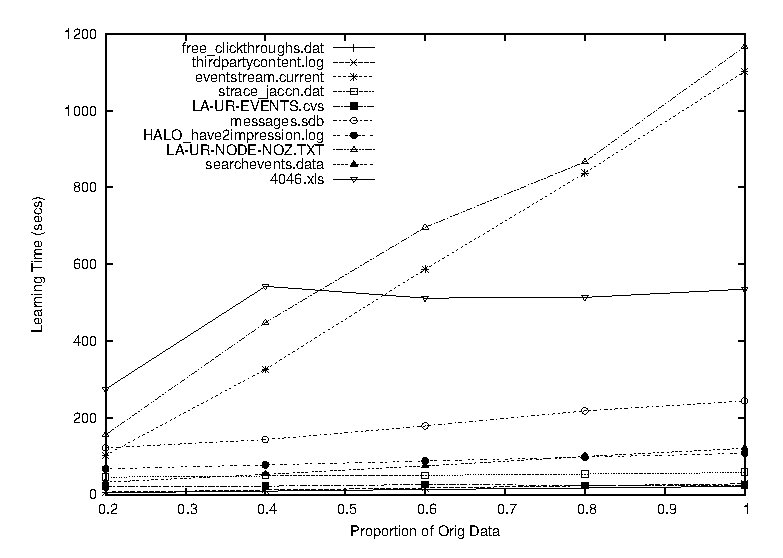
\includegraphics[width=\columnwidth]{scale-default}
%%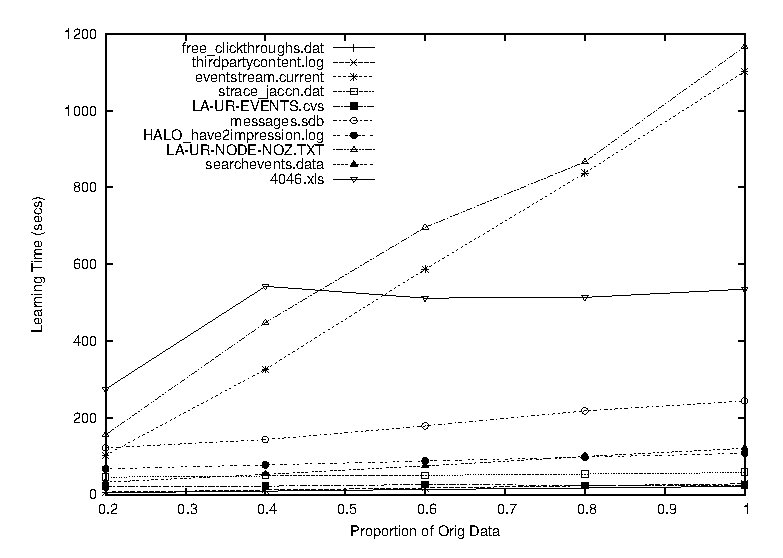
\epsfig{file=scale-default.eps, width=\columnwidth}
%\caption{Scaling Results with Default Settings}
%\end{figure}

\subsection{Scaling performance}
In the next experiment, we evaluate how the algorithm scales with increasing data size by running
the system on increasingly large fractions of each of the small data files, starting with 20\% and ending with 100\%.
For a given data source, we empirically determined which values of the batch-size parameters $N$ and $M$ give the best result when learning the entire source, 
and then used those values for this experiment.  
\figref{fig:scale} plots the resulting total learning time versus the 
percentage of the data file used in learning.   
The graph shows the algorithm enjoys
near linear scale-up for all sources except \cd{4046.xls}, which flattens after 40\% of
data.  The \emph{BlobFinding} rule is the cause of this anomaly: learning the initial description takes a relatively long time, but after the algorithm sees the first 40\% of the data, the \emph{BlobFinding} rule simplifies the description to one that parses much more quickly and correctly parses the rest of the data.  

\cut{
The cause of this anomaly is its small size relative to its complexity. 
Learning the initial description takes a lot of time.
After the algorithm learns the first 40\% of the data, the description was updated to a
fairly simply one due to \cd{BlobFinding}. Parsing the remaining data resulted in no
additional errors and took minimal further time. }

\begin{figure}[t]
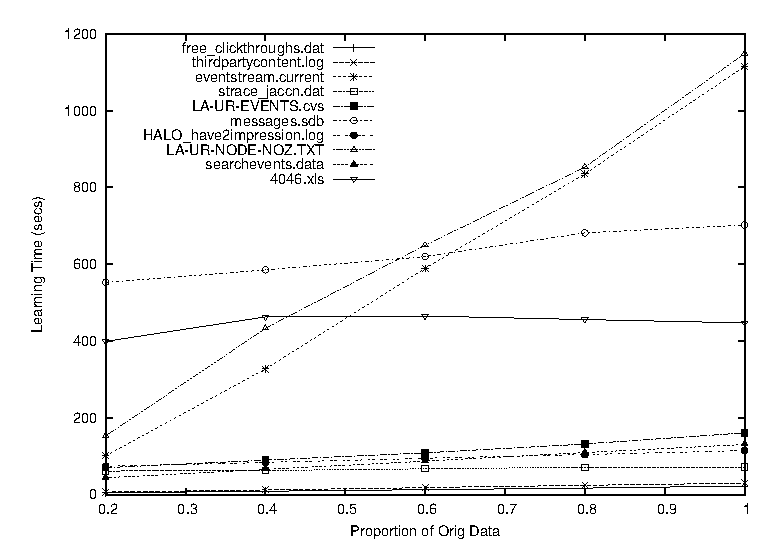
\includegraphics[width=\columnwidth]{scale-uc}
%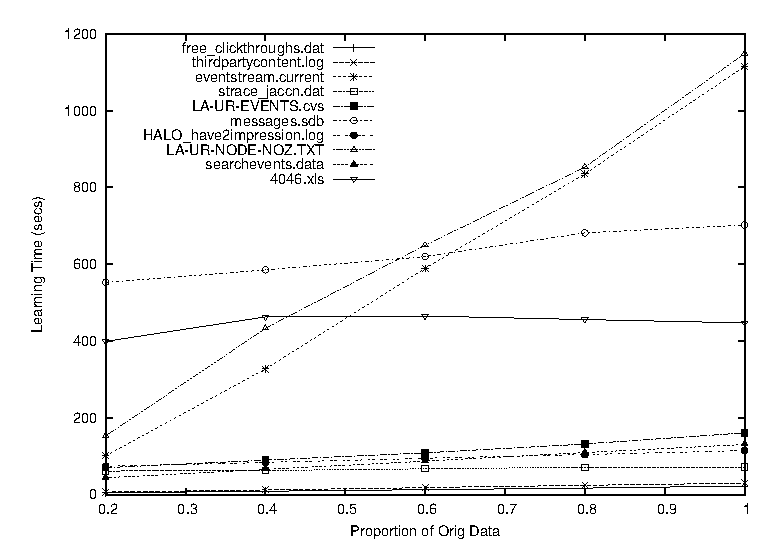
\epsfig{file=scale-uc.eps, width=\columnwidth}
\caption{Learning time vs percentage of data sources}
\vskip -2ex
\label{fig:scale}
\end{figure}


\cut{%%% DPW: cut the union clustering section.
\cut{%%%%%%%%%  the following table has a score column %%%%%%%%%%%
\begin{table*}[th]
\centering
\caption{Without Union Clustering vs. With Union Clustering}
\label{tab:uceffects}
\begin{tabular}{|c||c|c||c|c||c|c|} \hline
 & Time & Time (UC) & Score & Score(UC) & Dist & Dist (UC) \\ \hline \hline
free\_clickthroughs.dat & 23.81  & {\bf 23.41} & 5275.94 & 5275.94 & 0.19 & 0.19 \\ \hline
thirdpartycontent.log & 38.29 & {\bf 28.23} & {\bf 9041.38} & 9041.41 & 0.55 & 0.55 \\ \hline
eventstream.current & {\bf 1129.86} & 1286.60 & {\bf 14949.20} & 15184.53 & 5.32 & {\bf 5.05} \\ \hline
strace\_jaccn.dat & 235.47 & {\bf 232.27} & 7381.82 & 7381.82 & 0.26 & 0.26 \\ \hline
LA-UR-EVENTS.csv & {\bf 57.90} & 66.58 & {\bf 5637.25} & 6065.06 & 1.33 & {\bf 1.27} \\ \hline
messages.sdb & {\bf 125.42} & 127.76 & 8098.46 & 8096.46 & 0.67 & 0.67 \\ \hline
HALO\_have2impression.log & 122.33 & {\bf 121.75} & 25051.52 & 25051.52 & 1.59 & 1.59 \\ \hline
LA-UR-NODE-NOZ.TXT & {\bf 1154.12} & 1185.79 & 10572.83 & 10572.83 & 0.59 & 0.59 \\ \hline
searchevents.dat & {\bf 4300.79} & 6890.45 & 16650.63 & {\bf 16529.90} & {\bf 2.33} & 2.39 \\ \hline
4046.xls & 15.20 & {\bf 13.57} & 22549.14 & 22549.14 & 0.99 & 0.99  \\ \hline
%smallrace.log & 19.74 & 42782.44 & 0.97 & 19.66 & 42779.64 & NA \\ \hline
\end{tabular}
}%%%%%%%%%%%%%%% end of cut %%%%%%%%%%%%%%%


\begin{table}[th]
\centering
\caption{Default vs. Union Clustering}
\label{tab:uceffects}
\begin{tabular}{|c||c|c||c|c|} \hline
\multirow{2}{*}{Sources} & \multicolumn{2}{c||}{Time(sec)} & \multicolumn{2}{c|}{Dist} \\ \cline{2-5}
 & Def & UC &  Def & UC \\ \hline 
free\_clickthroughs.dat & 23.81  & {\bf 23.41} & 0.19 & 0.19 \\ \hline
thirdpartycontent.log & 38.29 & {\bf 28.23} & 0.55 & 0.55 \\ \hline
eventstream.current & {\bf 1129.86} & 1286.60 & 5.32 & {\bf 5.05} \\ \hline
strace\_jaccn.dat & 235.47 & {\bf 232.27} & 0.26 & 0.26 \\ \hline
LA-UR-EVENTS.csv & {\bf 57.90} & 66.58 & 1.33 & {\bf 1.27} \\ \hline
messages.sdb & {\bf 125.42} & 127.76 & 0.67 & 0.67 \\ \hline
HALO\_have2impression.log & 122.33 & {\bf 121.75} & 1.59 & 1.59 \\ \hline
LA-UR-NODE-NOZ.TXT & {\bf 1154.12} & 1185.79 & 0.59 & 0.59 \\ \hline
searchevents.dat & {\bf 4300.79} & 6890.45 & {\bf 2.33} & 2.39 \\ \hline
4046.xls & 15.20 & {\bf 13.57} & 0.99 & 0.99  \\ \hline
%smallrace.log & 19.74 & 42782.44 & 0.97 & 19.66 & 42779.64 & NA \\ \hline
\end{tabular}
\end{table}

\subsection{Union clustering or not?}
In this experiment, we contrast the performance of the system with and without
union clustering in the \learnpads{} algorithm for 10 small files in 
Table \ref{tab:uceffects}. We learned the initial description using the
the first 500 records in each of these files and set the
incremental batch size $M$ to be 100. We conclude that
union clustering helps produce more human readable descriptions with shallower
nesting and hence the distance score is better in two of the ten sources by
quite a large margin. Moreover, this can be achieved without spending much 
more time. Therefore, we turned on union clustering feature in the remaining
experiments below. 
}

\subsection{Initial and incremental batch size}
\cut{%%%%%%%%%%%%%%%%%%%%%%%%%%%%

\subsubsection{Default settings}

\begin{table}[th]
\caption{free\_clickthroughs.dat.cleaned}
\label{tab:free_clickthroughs.dat.cleaned}
\centering
\begin{tabular}{|c||c|c|c|c|c|}
\hline
init/inc & 25 & 100 & 400 & 1600 & 6400 \\ \hline \hline
  & 22.06 & 23.81 & 33.60 & 43.50 & 43.16\\ 
500  & 5275.94 & 5275.94 & 5275.94 & 5275.94 & 5275.94\\ 
  & 0.19 & 0.19 & 0.19 & 0.19 & 0.19\\ \hline 
  & 21.84 & 24.12 & 33.77 & 43.59 & 45.75\\ 
1000  & 5275.94 & 5275.94 & 5275.94 & 5275.94 & 5275.94\\ 
  & 0.19 & 0.19 & 0.19 & 0.19 & 0.19\\ \hline 
  & 21.27 & 22.37 & 21.38 & 20.94 & 22.22\\ 
2000  & 5275.94 & 5275.94 & 5275.94 & 5275.94 & 5275.94\\ 
  & 0.19 & 0.19 & 0.19 & 0.19 & 0.19\\ \hline 
  & 21.68 & 21.63 & 21.75 & 21.85 & 21.70\\ 
4000  & 5272.57 & 5272.57 & 5272.57 & 5272.57 & 5272.57\\ 
  & 0.19 & 0.19 & 0.19 & 0.19 & 0.19\\ \hline 
  & 24.11 & 24.14 & 24.41 & 24.26 & 24.38\\ 
8000  & 5272.57 & 5272.57 & 5272.57 & 5272.57 & 5272.57\\ 
  & 0.19 & 0.19 & 0.19 & 0.19 & 0.19\\ \hline 
  & 37.86 & 39.15 & 37.36 & 37.94 & 37.48\\ 
16000  & 5272.57 & 5272.57 & 5272.57 & 5272.57 & 5272.57\\ 
  & 0.19 & 0.19 & 0.19 & 0.19 & 0.19\\ \hline 
  & 113.83 & 107.79 & 109.23 & 107.75 & 107.70\\ 
32000  & 5272.57 & 5272.57 & 5272.57 & 5272.57 & 5272.57\\ 
  & 0.19 & 0.19 & 0.19 & 0.19 & 0.19\\ \hline 
  & 510.99 & 510.04 & 531.80 & 510.24 & 534.57\\ 
64000  & 5272.57 & 5272.57 & 5272.57 & 5272.57 & 5272.57\\ 
  & 0.19 & 0.19 & 0.19 & 0.19 & 0.19\\ \hline 
\end{tabular}
\end{table}

\begin{table}[th]
\caption{thirdpartycontent.log}
\label{tab:thirdpartycontent.log}
\centering
\begin{tabular}{|c||c|c|c|c|c|}
\hline
init/inc & 25 & 100 & 400 & 1600 & 6400 \\ \hline \hline
  & 39.04 & 38.29 & 38.54 & 38.86 & 38.75\\ 
500  & 9041.38 & 9041.38 & 9041.38 & 9041.38 & 9041.38\\ 
  & 0.55 & 0.55 & 0.55 & 0.55 & 0.55\\ \hline 
  & 67.64 & 67.42 & 67.45 & 67.71 & 67.25\\ 
1000  & 9560.76 & 9560.76 & 9560.76 & 9560.76 & 9560.76\\ 
  & 1.20 & 1.20 & 1.20 & 1.20 & 1.20\\ \hline 
  & 28.82 & 28.83 & 28.84 & 28.64 & 28.75\\ 
2000  & 9038.22 & 9038.22 & 9038.22 & 9038.22 & 9038.22\\ 
  & 0.55 & 0.55 & 0.55 & 0.55 & 0.55\\ \hline 
  & 31.72 & 31.47 & 31.48 & 31.67 & 31.52\\ 
4000  & 9038.22 & 9038.22 & 9038.22 & 9038.22 & 9038.22\\ 
  & 0.55 & 0.55 & 0.55 & 0.55 & 0.55\\ \hline 
  & 37.77 & 35.83 & 35.61 & 35.62 & 35.55\\ 
8000  & 9038.22 & 9038.22 & 9038.22 & 9038.22 & 9038.22\\ 
  & 0.55 & 0.55 & 0.55 & 0.55 & 0.55\\ \hline 
  & 92.91 & 91.30 & 92.36 & 94.59 & 93.65\\ 
16000  & 9038.22 & 9038.22 & 9038.22 & 9038.22 & 9038.22\\ 
  & 0.55 & 0.55 & 0.55 & 0.55 & 0.55\\ \hline 
  & 231.29 & 227.22 & 235.68 & 251.48 & 241.52\\ 
32000  & 9038.22 & 9038.22 & 9038.22 & 9038.22 & 9038.22\\ 
  & 0.55 & 0.55 & 0.55 & 0.55 & 0.55\\ \hline 
  & 899.51 & 888.39 & 895.54 & 888.73 & 886.84\\ 
64000  & 9038.22 & 9038.22 & 9038.22 & 9038.22 & 9038.22\\ 
  & 0.55 & 0.55 & 0.55 & 0.55 & 0.55\\ \hline 
\end{tabular}
\end{table}


\begin{table}[th]
\caption{eventstream.current}
\label{tab:eventstream.current}
\centering
\begin{tabular}{|c||c|c|c|c|c|}
\hline
init/inc & 25 & 100 & 400 & 1600 & 6400 \\ \hline \hline
       & 454.17   & 806.17  & 889.54  & 1046.30 & 855.84 \\
Manual & 10199.04 & 9763.39 & 9763.39 & 9767.39 & 9742.43 \\
       & 3.37     & 3.00    & 3.00    & 3.00    & 3.00 \\ \hline
  & 771.56 & 1129.86 & 1064.14 & 1064.82 & 1079.70\\ 
500  & 16016.90 & 14949.20 & 14949.20 & 14949.20 & 14949.20\\ 
  & 6.47 & 5.32 & 5.32 & 5.32 & 5.32\\ \hline 
  & 764.72 & 1126.15 & 1121.27 & 1105.52 & 1106.83\\ 
1000  & 15816.19 & 15184.35 & 15184.35 & 15184.35 & 15184.35\\ 
  & 5.32 & 5.05 & 5.05 & 5.05 & 5.05\\ \hline 
  & 747.93 & 1116.85 & 1098.70 & 1105.55 & 1110.98\\ 
2000  & 15815.83 & 15183.99 & 15183.99 & 15183.99 & 15183.99\\ 
  & 5.32 & 5.05 & 5.05 & 5.05 & 5.05\\ \hline 
  & 1227.79 & 1110.77 & 1109.46 & 1102.75 & 1115.54\\ 
4000  & 16475.50 & 15460.89 & 15460.89 & 15460.89 & 15460.89\\ 
  & 6.79 & 5.74 & 5.74 & 5.74 & 5.74\\ \hline 
  & 1244.07 & 1130.73 & 1137.79 & 1125.92 & 1137.29\\ 
8000  & 16474.98 & 15460.37 & 15460.37 & 15460.37 & 15460.37\\ 
  & 6.79 & 5.74 & 5.74 & 5.74 & 5.74\\ \hline 
  & 1363.05 & 1262.70 & 1303.50 & 1262.10 & 1295.53\\ 
16000  & 16473.96 & 15459.34 & 15459.34 & 15459.34 & 15459.34\\ 
  & 6.79 & 5.74 & 5.74 & 5.74 & 5.74\\ \hline 
  &  &  &  &  & \\ 
32000  &  &  &  &  & \\ 
  &  &  &  &  & \\ \hline 
  &  &  &  &  & \\ 
64000  &  &  &  &  & \\ 
  &  &  &  &  & \\ \hline 
\end{tabular}
\end{table}

\begin{table}[th]
\caption{strace\_jaccn.dat}
\label{tab:strace_jaccn.dat}
\centering
\begin{tabular}{|c||c|c|c|c|c|}
\hline
init/inc & 25 & 100 & 400 & 1600 & 6400 \\ \hline \hline
  & 235.59 & 235.47 & 237.31 & 238.53 & 237.49\\ 
500  & 7381.82 & 7381.82 & 7381.82 & 7381.82 & 7381.82\\ 
  & 0.26 & 0.26 & 0.26 & 0.26 & 0.26\\ \hline 
  & 236.30 & 243.02 & 241.56 & 246.84 & 241.23\\ 
1000  & 7381.36 & 7381.36 & 7381.36 & 7381.36 & 7381.36\\ 
  & 0.26 & 0.26 & 0.26 & 0.26 & 0.26\\ \hline 
  & 58.09 & 58.22 & 58.74 & 57.56 & 58.80\\ 
2000  & 7246.68 & 7246.68 & 7246.68 & 7246.68 & 7246.68\\ 
  & 0.12 & 0.12 & 0.12 & 0.12 & 0.12\\ \hline 
  & 52.54 & 52.88 & 52.80 & 52.98 & 52.81\\ 
4000  & 7286.71 & 7286.71 & 7286.71 & 7286.71 & 7286.71\\ 
  & 0.15 & 0.15 & 0.15 & 0.15 & 0.15\\ \hline 
  & 177.43 & 177.71 & 195.38 & 177.78 & 177.62\\ 
8000  & 7278.96 & 7278.96 & 7278.96 & 7278.96 & 7278.96\\ 
  & 0.15 & 0.15 & 0.15 & 0.15 & 0.15\\ \hline 
  & 1716.79 & 1708.83 & 1798.74 & 1707.60 & 1705.33\\ 
16000  & 9337.44 & 9337.44 & 9337.44 & 9337.44 & 9337.44\\ 
  & 1.19 & 1.19 & 1.19 & 1.19 & 1.19\\ \hline 
  &  &  &  &  & \\ 
32000  &  &  &  &  & \\ 
  &  &  &  &  & \\ \hline 
  &  &  &  &  & \\ 
64000  &  &  &  &  & \\ 
  &  &  &  &  & \\ \hline 
\end{tabular}
\end{table}

\begin{table}[th]
\caption{LA-UR-06-0803-MX20\_NODES\_0\_TO\_255\_EVENTS.csv}
\label{tab:LA-UR-06-0803-MX20_NODES_0_TO_255_EVENTS.csv}
\centering
\begin{tabular}{|c||c|c|c|c|c|}
\hline
init/inc & 25 & 100 & 400 & 1600 & 6400 \\ \hline \hline
  & 62.40 & 57.90 & 58.58 & 69.14 & 110.47\\ 
500  & 5666.51 & 5637.25 & 5637.25 & 5701.30 & 5701.24\\ 
  & 1.33 & 1.33 & 1.33 & 1.33 & 1.33\\ \hline 
  & 62.33 & 63.90 & 65.74 & 75.22 & 364.57\\ 
1000  & 6122.50 & 6186.65 & 6186.63 & 6186.27 & 7370.52\\ 
  & 1.13 & 1.13 & 1.13 & 1.13 & 2.27\\ \hline 
  & 27.48 & 24.50 & 25.19 & 32.65 & 153.22\\ 
2000  & 5773.51 & 5773.51 & 5773.51 & 5773.51 & 5773.51\\ 
  & 0.67 & 0.67 & 0.67 & 0.67 & 0.67\\ \hline 
  & 25.25 & 25.27 & 25.99 & 29.67 & 93.97\\ 
4000  & 5773.51 & 5773.51 & 5773.51 & 5773.51 & 5773.51\\ 
  & 0.67 & 0.67 & 0.67 & 0.67 & 0.67\\ \hline 
  & 24.25 & 25.60 & 24.78 & 27.05 & 279.74\\ 
8000  & 5773.51 & 5773.51 & 5773.51 & 5773.51 & 8259.43\\ 
  & 0.67 & 0.67 & 0.67 & 0.67 & 6.93\\ \hline 
  & 46.98 & 45.18 & 45.68 & 48.29 & 314.31\\ 
16000  & 5773.51 & 5773.51 & 5773.51 & 5773.51 & 8259.43\\ 
  & 0.67 & 0.67 & 0.67 & 0.67 & 6.93\\ \hline 
  & 194.77 & 195.67 & 195.41 & 197.24 & 197.77\\ 
32000  & 6121.86 & 6186.01 & 6185.99 & 6185.62 & 6183.36\\ 
  & 1.13 & 1.13 & 1.13 & 1.13 & 1.13\\ \hline 
  &  &  &  &  & \\ 
64000  &  &  &  &  & \\ 
  &  &  &  &  & \\ \hline 
\end{tabular}
\end{table}

\begin{table}[th]
\caption{messages.sdb}
\label{tab:messages.sdb}
\centering
\begin{tabular}{|c||c|c|c|c|c|}
\hline
init/inc & 25 & 100 & 400 & 1600 & 6400 \\ \hline \hline
       & 294.11     & 398.34   & 347.50   & 291.33   & 290.55 \\
Manual & 8316.77    & 8355.71  & 8313.52  & 8297.47  & 8297.47 \\
       & 0.62       & 0.62     & 0.62     & 0.52     & 0.52 \\ \hline
  & 127.38 & 125.42 & 124.59 & 124.49 & 138.14\\ 
500  & 8098.46 & 8098.46 & 8098.46 & 8098.46 & 8098.46\\ 
  & 0.67 & 0.67 & 0.67 & 0.67 & 0.67\\ \hline 
  & 442.05 & 419.83 & 435.06 & 514.53 & 456.84\\ 
1000  & 9346.35 & 8443.28 & 8549.67 & 8544.63 & 8541.95\\ 
  & 1.10 & 1.10 & 1.24 & 1.24 & 1.24\\ \hline 
  & 3833.25 & 3723.05 & 3873.68 & 3690.93 & 3707.39\\ 
2000  & 10785.36 & 10785.36 & 10785.36 & 10785.36 & 10785.36\\ 
  & 2.24 & 2.24 & 2.24 & 2.24 & 2.24\\ \hline 
  & 895.22 & 894.24 & 959.23 & 933.91 & 949.04\\ 
4000  & 7936.66 & 7936.66 & 7936.66 & 7936.66 & 7936.66\\ 
  & 0.57 & 0.57 & 0.57 & 0.57 & 0.57\\ \hline 
  & 245.00 & 242.51 & 244.41 & 242.07 & 241.57\\ 
8000  & 7895.66 & 7895.66 & 7895.66 & 7895.66 & 7895.66\\ 
  & 0.52 & 0.52 & 0.52 & 0.52 & 0.52\\ \hline 
  & 741.59 & 776.98 & 735.58 & 756.83 & 740.93\\ 
16000  & 7895.61 & 7895.61 & 7895.61 & 7895.61 & 7895.61\\ 
  & 0.52 & 0.52 & 0.52 & 0.52 & 0.52\\ \hline 
  &  &  &  &  & \\ 
32000  &  &  &  &  & \\ 
  &  &  &  &  & \\ \hline 
  &  &  &  &  & \\ 
64000  &  &  &  &  & \\ 
  &  &  &  &  & \\ \hline 
\end{tabular}
\end{table}

\begin{table}[th]
\caption{HALO\_have2impression.log.1}
\label{tab:HALO_have2impression.log.1}
\centering
\begin{tabular}{|c||c|c|c|c|c|}
\hline
init/inc & 25 & 100 & 400 & 1600 & 6400 \\ \hline \hline
  & 120.11 & 122.33 & 72.75 & 84.45 & 238.90\\ 
500  & 25051.52 & 25051.52 & 22492.36 & 22492.36 & 22478.79\\ 
  & 1.59 & 1.59 & 1.00 & 1.00 & 0.97\\ \hline 
  & 380.55 & 103.51 & 383.83 & 69.75 & 143.48\\ 
1000  & 118131.33 & 33519.25 & 34205.86 & 32943.53 & 32703.57\\ 
  & 4.06 & 1.12 & 4.32 & 0.82 & 0.82\\ \hline 
  & 30.81 & 36.33 & 175.08 & 31.30 & 273.48\\ 
2000  & 32056.85 & 32056.84 & 31351.37 & 32058.39 & 30935.61\\ 
  & 0.76 & 0.76 & 9.24 & 0.76 & 10.29\\ \hline 
  & 72.27 & 72.32 & 72.49 & 72.27 & 72.32\\ 
4000  & 27464.99 & 27464.99 & 27464.99 & 27464.99 & 27464.99\\ 
  & 0.65 & 0.65 & 0.65 & 0.65 & 0.65\\ \hline 
  & 108.12 & 107.92 & 108.14 & 107.95 & 108.19\\ 
8000  & 27460.96 & 27460.96 & 27460.96 & 27460.96 & 27460.96\\ 
  & 0.65 & 0.65 & 0.65 & 0.65 & 0.65\\ \hline 
  & 258.59 & 258.53 & 258.68 & 259.21 & 258.59\\ 
16000  & 28208.58 & 28208.58 & 28208.58 & 28208.58 & 28208.58\\ 
  & 1.15 & 1.15 & 1.15 & 1.15 & 1.15\\ \hline 
  &  &  &  &  & \\ 
32000  &  &  &  &  & \\ 
  &  &  &  &  & \\ \hline 
  &  &  &  &  & \\ 
64000  &  &  &  &  & \\ 
  &  &  &  &  & \\ \hline 
\end{tabular}
\end{table}

\begin{table}[th]
\caption{LA-UR-06-1446-MX16-NODE-NOZ.TXT}
\label{tab:LA-UR-06-1446-MX16-NODE-NOZ.TXT}
\centering
\begin{tabular}{|c||c|c|c|c|c|}
\hline
init/inc & 25 & 100 & 400 & 1600 & 6400 \\ \hline \hline
  & 1180.88 & 1154.12 & 1169.15 & 1154.12 & 1159.82\\ 
500  & 10572.83 & 10572.83 & 10572.83 & 10572.83 & 10572.83\\ 
  & 0.59 & 0.59 & 0.59 & 0.59 & 0.59\\ \hline 
  & 157.06 & 185.63 & 123.20 & 141.03 & 306.10\\ 
1000  & 13649.76 & 13649.76 & 13977.36 & 13977.36 & 13977.36\\ 
  & 0.67 & 0.67 & 0.65 & 0.65 & 0.65\\ \hline 
  & 779.84 & 782.27 & 790.20 & 786.88 & 814.10\\ 
2000  & 10652.04 & 13059.61 & 10954.11 & 10954.11 & 10954.11\\ 
  & 0.71 & 0.73 & 0.78 & 0.78 & 0.78\\ \hline 
  & 1501.05 & 1564.35 &  &  & \\ 
4000  & 10422.70 & 12035.14 &  &  & \\ 
  & 0.76 & 0.78 &  &  & \\ \hline 
  & 1661.94 & 1641.32 &  &  & \\ 
8000  & 8289.28 & 12210.88 &  &  & \\ 
  & 0.82 & 0.86 &  &  & \\ \hline 
  &  &  &  &  & \\ 
16000  &  &  &  &  & \\ 
  &  &  &  &  & \\ \hline 
  &  &  &  &  & \\ 
32000  &  &  &  &  & \\ 
  &  &  &  &  & \\ \hline 
  &  &  &  &  & \\ 
64000  &  &  &  &  & \\ 
  &  &  &  &  & \\ \hline 
\end{tabular}
\end{table}

\begin{table}[th]
\caption{searchevents.dat.cleaned}
\label{tab:searchevents.dat.cleaned}
\centering
\begin{tabular}{|c||c|c|c|c|c|}
\hline
init/inc & 25 & 100 & 400 & 1600 & 6400 \\ \hline \hline
  & 2649.60 & 4300.79 & 5921.21 & 18424.27 & \\ 
500  & 13723.05 & 16650.63 & 17368.35 & 17810.89 & \\ 
  & 1.82 & 2.33 & 4.05 & 3.64 & \\ \hline 
  &  &  &  &  & \\ 
1000  &  &  &  &  & \\ 
  &  &  &  &  & \\ \hline 
  & 122.22 & 120.48 & 117.97 & 120.80 & 118.36\\ 
2000  & 12779.72 & 12779.72 & 12779.72 & 12779.72 & 12779.72\\ 
  & 0.84 & 0.84 & 0.84 & 0.84 & 0.84\\ \hline 
  & 134.70 & 134.48 & 134.30 & 132.09 & 134.13\\ 
4000  & 12778.65 & 12778.65 & 12778.65 & 12778.65 & 12778.65\\ 
  & 0.84 & 0.84 & 0.84 & 0.84 & 0.84\\ \hline 
  &  &  &  &  & \\ 
8000  &  &  &  &  & \\ 
  &  &  &  &  & \\ \hline 
  &  &  &  &  & \\ 
16000  &  &  &  &  & \\ 
  &  &  &  &  & \\ \hline 
  &  &  &  &  & \\ 
32000  &  &  &  &  & \\ 
  &  &  &  &  & \\ \hline 
  &  &  &  &  & \\ 
64000  &  &  &  &  & \\ 
  &  &  &  &  & \\ \hline 
\end{tabular}
\end{table}

\begin{table}[th]
\caption{4046.xls}
\label{tab:4046.xls}
\centering
\begin{tabular}{|c||c|c|c|c|c|}
\hline
init/inc & 25 & 100 & 400 & 1600 & 6400 \\ \hline \hline
  & 14.49 & 15.20 & 14.47 & 14.69 & 14.67\\ 
500  & 22549.14 & 22549.14 & 22549.14 & 22549.14 & 22549.14\\ 
  & 0.99 & 0.99 & 0.99 & 0.99 & 0.99\\ \hline 
  & 111.41 & 182.24 & 385.50 & 888.66 & 884.30\\ 
1000  & 22551.31 & 22144.76 & 20994.62 & 18312.58 & 18312.58\\ 
  & 1.00 & 1.00 & 1.00 & 1.00 & 1.00\\ \hline 
  & 102.85 & 131.20 & 455.85 &  & \\ 
2000  & 22403.55 & 22338.03 & 22107.26 &  & \\ 
  & 0.98 & 0.98 & 0.98 &  & \\ \hline 
  &  &  &  &  & \\ 
4000  &  &  &  &  & \\ 
  &  &  &  &  & \\ \hline 
  & 588.85 & 590.57 & 588.47 & 589.98 & \\ 
8000  & 22829.02 & 22829.02 & 22829.02 & 22829.02 & \\ 
  & 0.97 & 0.97 & 0.97 & 0.97 & \\ \hline 
  &  &  &  &  & \\ 
16000  &  &  &  &  & \\ 
  &  &  &  &  & \\ \hline 
  &  &  &  &  & \\ 
32000  &  &  &  &  & \\ 
  &  &  &  &  & \\ \hline 
  &  &  &  &  & \\ 
64000  &  &  &  &  & \\ 
  &  &  &  &  & \\ \hline 
\end{tabular}
\end{table}
\cleardoublepage

\subsubsection{With union clustering}
\begin{table}[th]
\caption{free\_clickthroughs.dat.cleaned}
\label{tab:free_clickthroughs.dat.cleaned}
\centering
\begin{tabular}{|c||c|c|c|c|c|}
\hline
init/inc & 25 & 100 & 400 & 1600 & 6400 \\ \hline \hline
  & 21.44 & 23.41 & 32.69 & 42.11 & 42.18\\ 
500  & 5275.94 & 5275.94 & 5275.94 & 5275.94 & 5275.94\\ 
  & 0.19 & 0.19 & 0.19 & 0.19 & 0.19\\ \hline 
  & 21.37 & 23.39 & 32.87 & 42.42 & 42.29\\ 
1000  & 5275.94 & 5275.94 & 5275.94 & 5275.94 & 5275.94\\ 
  & 0.19 & 0.19 & 0.19 & 0.19 & 0.19\\ \hline 
  & 20.71 & 20.71 & 20.70 & 20.74 & 20.73\\ 
2000  & 5275.94 & 5275.94 & 5275.94 & 5275.94 & 5275.94\\ 
  & 0.19 & 0.19 & 0.19 & 0.19 & 0.19\\ \hline 
  & 21.20 & 21.15 & 21.18 & 21.14 & 21.21\\ 
4000  & 5272.57 & 5272.57 & 5272.57 & 5272.57 & 5272.57\\ 
  & 0.19 & 0.19 & 0.19 & 0.19 & 0.19\\ \hline 
  & 23.81 & 23.73 & 23.90 & 23.79 & 23.72\\ 
8000  & 5272.57 & 5272.57 & 5272.57 & 5272.57 & 5272.57\\ 
  & 0.19 & 0.19 & 0.19 & 0.19 & 0.19\\ \hline 
  & 36.52 & 36.47 & 36.50 & 36.48 & 36.50\\ 
16000  & 5272.57 & 5272.57 & 5272.57 & 5272.57 & 5272.57\\ 
  & 0.19 & 0.19 & 0.19 & 0.19 & 0.19\\ \hline 
  & 105.16 & 105.14 & 105.27 & 105.26 & 105.10\\ 
32000  & 5272.57 & 5272.57 & 5272.57 & 5272.57 & 5272.57\\ 
  & 0.19 & 0.19 & 0.19 & 0.19 & 0.19\\ \hline 
  & 501.44 & 501.24 & 502.60 & 501.60 & 500.86\\ 
64000  & 5272.57 & 5272.57 & 5272.57 & 5272.57 & 5272.57\\ 
  & 0.19 & 0.19 & 0.19 & 0.19 & 0.19\\ \hline 
\end{tabular}
\end{table}

\begin{table}[th]
\caption{thirdpartycontent.log}
\label{tab:thirdpartycontent.log}
\centering
\begin{tabular}{|c||c|c|c|c|c|}
\hline
init/inc & 25 & 100 & 400 & 1600 & 6400 \\ \hline \hline
  & 27.54 & 28.23 & 39.19 & 92.23 & 276.86\\ 
500  & 9041.41 & 9041.41 & 9041.41 & 9041.40 & 9041.37\\ 
  & 0.55 & 0.55 & 0.55 & 0.55 & 0.55\\ \hline 
  & 56.99 & 55.88 & 63.67 & 124.97 & 350.59\\ 
1000  & 9560.79 & 9560.79 & 9560.79 & 9560.78 & 9560.75\\ 
  & 1.20 & 1.20 & 1.20 & 1.20 & 1.20\\ \hline 
  & 28.14 & 28.11 & 28.16 & 28.27 & 28.10\\ 
2000  & 9038.22 & 9038.22 & 9038.22 & 9038.22 & 9038.22\\ 
  & 0.55 & 0.55 & 0.55 & 0.55 & 0.55\\ \hline 
  & 30.89 & 30.93 & 31.00 & 30.93 & 30.82\\ 
4000  & 9038.22 & 9038.22 & 9038.22 & 9038.22 & 9038.22\\ 
  & 0.55 & 0.55 & 0.55 & 0.55 & 0.55\\ \hline 
  & 34.97 & 34.93 & 34.97 & 34.85 & 34.83\\ 
8000  & 9038.22 & 9038.22 & 9038.22 & 9038.22 & 9038.22\\ 
  & 0.55 & 0.55 & 0.55 & 0.55 & 0.55\\ \hline 
  & 61.44 & 61.39 & 61.52 & 61.44 & 61.49\\ 
16000  & 9038.22 & 9038.22 & 9038.22 & 9038.22 & 9038.22\\ 
  & 0.55 & 0.55 & 0.55 & 0.55 & 0.55\\ \hline 
  & 282.77 & 279.79 & 283.30 & 279.95 & 297.45\\ 
32000  & 9038.22 & 9038.22 & 9038.22 & 9038.22 & 9038.22\\ 
  & 0.55 & 0.55 & 0.55 & 0.55 & 0.55\\ \hline 
  & 841.00 & 871.93 & 825.18 & 825.74 & 825.87\\ 
64000  & 9038.20 & 9038.20 & 9038.20 & 9038.20 & 9038.20\\ 
  & 0.55 & 0.55 & 0.55 & 0.55 & 0.55\\ \hline 
\end{tabular}
\end{table}
}%%%%%%%%%%%%%%%%%%%%%%%%% end of cut %%%%%%%%%%%%%%%

\cut{%%%%%%%%%%%%%%%%%%%%%%%%%%%%%%%%%%%

\begin{table}[th]
\caption{strace\_jaccn.dat}
\label{tab:strace_jaccn.dat}
\centering
\begin{tabular}{|c||c|c|c|c|c|}
\hline
init/inc & 25 & 100 & 400 & 1600 & 6400 \\ \hline \hline
  & 228.29 & 232.27 & 231.27 & 228.70 & 227.62\\ 
500  & 7381.82 & 7381.82 & 7381.82 & 7381.82 & 7381.82\\ 
  & 0.26 & 0.26 & 0.26 & 0.26 & 0.26\\ \hline 
  & 263.56 & 230.79 & 263.50 & 231.50 & 230.99\\ 
1000  & 7381.36 & 7381.36 & 7381.36 & 7381.36 & 7381.36\\ 
  & 0.26 & 0.26 & 0.26 & 0.26 & 0.26\\ \hline 
  & 73.36 & 83.70 & 73.20 & 73.48 & 83.09\\ 
2000  & 7246.68 & 7246.68 & 7246.68 & 7246.68 & 7246.68\\ 
  & 0.12 & 0.12 & 0.12 & 0.12 & 0.12\\ \hline 
  & 52.72 & 52.76 & 52.39 & 60.03 & 52.72\\ 
4000  & 7286.68 & 7286.68 & 7286.68 & 7286.68 & 7286.68\\ 
  & 0.15 & 0.15 & 0.15 & 0.15 & 0.15\\ \hline 
  & 118.68 & 135.00 & 135.43 & 119.17 & 118.57\\ 
8000  & 7278.93 & 7278.93 & 7278.93 & 7278.93 & 7278.93\\ 
  & 0.15 & 0.15 & 0.15 & 0.15 & 0.15\\ \hline 
  & 435.21 & 433.18 & 433.99 & 433.26 & 434.40\\ 
16000  & 6052.63 & 6052.63 & 6052.63 & 6052.63 & 6052.63\\ 
  & 0.13 & 0.13 & 0.13 & 0.13 & 0.13\\ \hline 
  &  &  &  &  & \\ 
32000  &  &  &  &  & \\ 
  &  &  &  &  & \\ \hline 
  &  &  &  &  & \\ 
64000  &  &  &  &  & \\ 
  &  &  &  &  & \\ \hline 
\end{tabular}
\end{table}

\begin{table}[th]
\caption{LA-UR-06-0803-MX20\_NODES\_0\_TO\_255\_EVENTS.csv}
\label{tab:LA-UR-06-0803-MX20_NODES_0_TO_255_EVENTS.csv}
\centering
\begin{tabular}{|c||c|c|c|c|c|}
\hline
init/inc & 25 & 100 & 400 & 1600 & 6400 \\ \hline \hline
  & 76.18 & 66.58 & 66.42 & 73.59 & 206.11\\ 
500  & 6137.54 & 6065.06 & 6065.06 & 6065.06 & 5772.12\\ 
  & 2.13 & 1.27 & 1.27 & 1.27 & 0.67\\ \hline 
  & 66.05 & 64.64 & 65.45 & 74.62 & 158.54\\ 
1000  & 6122.50 & 6122.50 & 6122.50 & 6122.50 & 5772.10\\ 
  & 1.13 & 1.13 & 1.13 & 1.13 & 0.67\\ \hline 
  & 25.32 & 24.32 & 25.22 & 32.41 & 155.69\\ 
2000  & 5773.51 & 5773.51 & 5773.51 & 5773.51 & 5773.51\\ 
  & 0.67 & 0.67 & 0.67 & 0.67 & 0.67\\ \hline 
  & 20.10 & 20.01 & 20.47 & 22.86 & 263.92\\ 
4000  & 5773.51 & 5773.51 & 5773.51 & 5773.51 & 8231.02\\ 
  & 0.67 & 0.67 & 0.67 & 0.67 & 6.93\\ \hline 
  & 28.15 & 28.29 & 28.66 & 31.20 & 274.85\\ 
8000  & 5773.51 & 5773.51 & 5773.51 & 5773.51 & 8231.02\\ 
  & 0.67 & 0.67 & 0.67 & 0.67 & 6.93\\ \hline 
  & 68.78 & 68.97 & 69.54 & 71.90 & 319.46\\ 
16000  & 5773.51 & 5773.51 & 5773.51 & 5773.51 & 8231.02\\ 
  & 0.67 & 0.67 & 0.67 & 0.67 & 6.93\\ \hline 
  & 205.29 & 203.49 & 204.49 & 203.94 & 193.12\\ 
32000  & 6121.86 & 6121.86 & 6121.86 & 6121.86 & 6156.75\\ 
  & 1.13 & 1.13 & 1.13 & 1.13 & 1.13\\ \hline 
  & 1222.82 &  &  &  & \\ 
64000  & 5778.32 &  &  &  & \\ 
  & 0.73 &  &  &  & \\ \hline 
\end{tabular}
\end{table}
}%%%%%%%%%%%%%%%%%%%% end of cut %%%%%%%%%%%%%%%%%

\cut{%%%%%%%%%%%%%%%%%%%%%%%%%
\begin{table}[th]
\caption{HALO\_have2impression.log.1}
\label{tab:HALO_have2impression.log.1}
\centering
\begin{tabular}{|c||c|c|c|c|c|}
\hline
init/inc & 25 & 100 & 400 & 1600 & 6400 \\ \hline \hline
  & 121.27 & 121.75 & 72.20 & 83.70 & 217.59\\ 
500  & 25051.52 & 25051.52 & 22492.36 & 22492.36 & 22478.79\\ 
  & 1.59 & 1.59 & 1.00 & 1.00 & 0.97\\ \hline 
  & 369.50 & 116.94 & 381.37 & 68.13 & 141.53\\ 
1000  & 118131.33 & 33519.25 & 34205.86 & 32943.53 & 32703.57\\ 
  & 4.06 & 1.12 & 4.32 & 0.82 & 0.82\\ \hline 
  & 31.41 & 36.58 & 175.78 & 31.40 & 271.90\\ 
2000  & 32056.85 & 32056.84 & 31351.37 & 32058.39 & 30935.61\\ 
  & 0.76 & 0.76 & 9.24 & 0.76 & 10.29\\ \hline 
  & 74.87 & 73.62 & 73.44 & 75.15 & 73.72\\ 
4000  & 27464.99 & 27464.99 & 27464.99 & 27464.99 & 27464.99\\ 
  & 0.65 & 0.65 & 0.65 & 0.65 & 0.65\\ \hline 
  & 116.17 & 114.09 & 116.08 & 114.14 & 114.09\\ 
8000  & 27460.96 & 27460.96 & 27460.96 & 27460.96 & 27460.96\\ 
  & 0.65 & 0.65 & 0.65 & 0.65 & 0.65\\ \hline 
  & 280.28 & 284.98 & 285.39 & 284.90 & 284.43\\ 
16000  & 28208.58 & 28208.58 & 28208.58 & 28208.58 & 28208.58\\ 
  & 1.15 & 1.15 & 1.15 & 1.15 & 1.15\\ \hline 
  & 1170.82 &  &  &  & \\ 
32000  & 27944.86 &  &  &  & \\ 
  & 1.15 &  &  &  & \\ \hline 
  &  &  &  &  & \\ 
64000  &  &  &  &  & \\ 
  &  &  &  &  & \\ \hline 
\end{tabular}
\end{table}

\begin{table}[th]
\caption{LA-UR-06-1446-MX16-NODE-NOZ.TXT}
\label{tab:LA-UR-06-1446-MX16-NODE-NOZ.TXT}
\centering
\begin{tabular}{|c||c|c|c|c|c|}
\hline
init/inc & 25 & 100 & 400 & 1600 & 6400 \\ \hline \hline
  & 1281.71 & 1185.79 & 1224.63 & 1162.16 & 1165.66\\ 
500  & 10572.83 & 10572.83 & 10572.83 & 10572.83 & 10572.83\\ 
  & 0.59 & 0.59 & 0.59 & 0.59 & 0.59\\ \hline 
  & 159.04 & 187.25 & 124.42 & 146.40 & 313.34\\ 
1000  & 13649.76 & 13649.76 & 13977.36 & 13977.36 & 13977.36\\ 
  & 0.67 & 0.67 & 0.65 & 0.65 & 0.65\\ \hline 
  & 785.99 & 804.44 & 795.74 & 795.10 & 807.12\\ 
2000  & 10652.03 & 13059.59 & 10954.10 & 10954.10 & 10954.10\\ 
  & 0.71 & 0.73 & 0.78 & 0.78 & 0.78\\ \hline 
  & 1474.60 & 1477.00 & 44382.14 &  & \\ 
4000  & 10422.70 & 12035.14 & 9277.02 &  & \\ 
  & 0.76 & 0.78 & 0.80 &  & \\ \hline 
  &  &  &  &  & \\ 
8000  &  &  &  &  & \\ 
  &  &  &  &  & \\ \hline 
  &  &  &  &  & \\ 
16000  &  &  &  &  & \\ 
  &  &  &  &  & \\ \hline 
  &  &  &  &  & \\ 
32000  &  &  &  &  & \\ 
  &  &  &  &  & \\ \hline 
  &  &  &  &  & \\ 
64000  &  &  &  &  & \\ 
  &  &  &  &  & \\ \hline 
\end{tabular}
\end{table}

\begin{table}[th]
\caption{searchevents.dat.cleaned}
\label{tab:searchevents.dat.cleaned}
\centering
\begin{tabular}{|c||c|c|c|c|c|}
\hline
init/inc & 25 & 100 & 400 & 1600 & 6400 \\ \hline \hline
  & 9226.15 & 6890.45 &  &  & \\ 
500  & 17864.64 & 16529.90 &  &  & \\ 
  & 2.70 & 2.39 &  &  & \\ \hline 
  &  &  &  &  & \\ 
1000  &  &  &  &  & \\ 
  &  &  &  &  & \\ \hline 
  & 130.84 & 118.82 & 120.73 & 120.17 & 118.84\\ 
2000  & 12779.72 & 12779.72 & 12779.72 & 12779.72 & 12779.72\\ 
  & 0.84 & 0.84 & 0.84 & 0.84 & 0.84\\ \hline 
  & 134.77 & 132.15 & 131.94 & 134.39 & 134.70\\ 
4000  & 12778.65 & 12778.65 & 12778.65 & 12778.65 & 12778.65\\ 
  & 0.84 & 0.84 & 0.84 & 0.84 & 0.84\\ \hline 
  &  &  &  &  & \\ 
8000  &  &  &  &  & \\ 
  &  &  &  &  & \\ \hline 
  &  &  &  &  & \\ 
16000  &  &  &  &  & \\ 
  &  &  &  &  & \\ \hline 
  &  &  &  &  & \\ 
32000  &  &  &  &  & \\ 
  &  &  &  &  & \\ \hline 
  &  &  &  &  & \\ 
64000  &  &  &  &  & \\ 
  &  &  &  &  & \\ \hline 
\end{tabular}
\end{table}

\begin{table}[th]
\caption{4046.xls}
\label{tab:4046.xls}
\centering
\begin{tabular}{|c||c|c|c|c|c|}
\hline
init/inc & 25 & 100 & 400 & 1600 & 6400 \\ \hline \hline
  & 13.69 & 13.57 & 13.57 & 13.46 & 13.51\\ 
500  & 22549.14 & 22549.14 & 22549.14 & 22549.14 & 22549.14\\ 
  & 0.99 & 0.99 & 0.99 & 0.99 & 0.99\\ \hline 
  & 125.68 & 214.68 & 483.99 & 1443.91 & 1462.13\\ 
1000  & 22550.81 & 22143.57 & 20990.58 & 18300.71 & 18300.71\\ 
  & 1.00 & 1.00 & 1.00 & 1.00 & 1.00\\ \hline 
  & 104.54 & 150.36 & 449.77 &  & \\ 
2000  & 22403.55 & 22338.03 & 22107.26 &  & \\ 
  & 0.98 & 0.98 & 0.98 &  & \\ \hline 
  &  &  &  &  & \\ 
4000  &  &  &  &  & \\ 
  &  &  &  &  & \\ \hline 
  & 594.60 &  & 597.12 & 591.70 & \\ 
8000  & 22829.02 &  & 22829.02 & 22829.02 & \\ 
  & 0.97 &  & 0.97 & 0.97 & \\ \hline 
  &  &  &  &  & \\ 
16000  &  &  &  &  & \\ 
  &  &  &  &  & \\ \hline 
  &  &  &  &  & \\ 
32000  &  &  &  &  & \\ 
  &  &  &  &  & \\ \hline 
  &  &  &  &  & \\ 
64000  &  &  &  &  & \\ 
  &  &  &  &  & \\ \hline 
\end{tabular}
\end{table}

\cleardoublepage
}%%%%%%%%%%%%%%%% end of cut %%%%%%%%%%%%%%%%%%%
\begin{table}[th]
\caption{$N$ vs. $M$ - eventstream.current}
\label{tab:eventstream.current}
\centering
\begin{tabular}{|c||c|c|c|c|c|}
\hline
$N$\textbackslash $M$& 25 & 100 & 400 & 1600 & 6400 \\ \hline \hline
       & 3.37     & 3.00    & 3.00    & 3.00    & 3.00 \\ 
Manual & 10199.04 & 9763.39 & 9763.39 & 9763.39 & 9742.43 \\
(3600) & 442.18  & 827.66  & 897.30 & 910.00 & 868.01 \\ \hline
     & 5.05 & 5.05 & 5.05 & 5.05 & 5.05\\
500  & 16119.06 & 15184.53 & 15184.53 & 15184.53 & 15184.53\\ 
(0.30)  & 927.84 & 1286.60 & 1117.60 & 1147.43 & 1118.18\\ \hline 
  & 5.05 & 5.05 & 5.05 & 5.05 & 5.05\\ 
1000  & 16118.88 & 15184.35 & 15184.35 & 15184.35 & 15184.35\\ 
(0.89)  & 962.74 & 1088.59 & 1086.97 & 1113.33 & 1115.03\\ \hline 
  & 5.05 & 5.05 & 5.05 & {\bf 5.05} & 5.05\\ 
2000  & 16118.52 & 15183.99 & 15183.99 & {\bf 15183.99} & 15183.99\\ 
(2.24)  & 934.40 & 1117.25 & 1120.37 & {\bf 1100.55} & 1114.62\\ \hline 
  & 5.37 & 5.37 & 5.37 & 5.37 & 5.37\\ 
4000  & 16577.07 & 15642.54 & 15642.54 & 15642.54 & 15642.54\\ 
(9.34)  & 1393.08 & 1089.47 & 1198.06 & 1127.42 & 1091.39\\ \hline 
  & 5.37 & 5.37 & 5.37 & 5.37 & 5.37\\ 
8000  & 16575.84 & 15641.31 & 15641.31 & 15641.31 & 15641.31\\ 
(36.63)  & 1404.10 & 1115.77 & 1115.64 & 1186.75 & 1250.11\\ \hline 
  & 5.37 & 5.37 & 5.37 & 5.37 & 5.37\\ 
16000  & 16573.39 & 15638.87 & 15638.87 & 15638.87 & 15638.87\\ 
(164.38)  & 1545.75 & 1457.71 & 1443.14 & 1252.26 & 1331.52\\ \hline 
%  &  &  &  &  & \\ 
%32000  &  &  &  &  & \\ 
%  &  &  &  &  & \\ \hline 
%  &  &  &  &  & \\ 
%64000  &  &  &  &  & \\ 
%  &  &  &  &  & \\ \hline 
\end{tabular}
\end{table}
\begin{table}[th]
\caption{$N$ vs. $M$ - messages.sdb}
\label{tab:messages.sdb}
\centering
\begin{tabular}{|c||c|c|c|c|c|}
\hline
$N$\textbackslash $M$& 25 & 100 & 400 & 1600 & 6400 \\ \hline \hline
       & 0.62    & 0.62    & 0.62    & 0.52    & 0.52  \\ 
Manual & 8316.77 & 8355.71 & 8313.52 & 8297.47 & 8297.04 \\
(3600) & 337.44  & 438.29  & 292.88  & 295.68  & 292.05 \\\hline
  & 0.67 & 0.67 & 0.67 & 0.67 & 0.67\\
500  & 8098.46 & 8098.46 & 8098.46 & 8098.46 & 8098.46\\ 
(2.13)  & 123.88 & 127.76 & 130.17 & 125.52 & 124.45\\ \hline 
  & 1.10 & 1.10 & 1.24 & 1.24 & 1.24\\ 
1000  & 9346.35 & 8443.28 & 8549.67 & 8544.63 & 8541.95\\ 
(5.75)  & 432.61 & 418.64 & 425.35 & 442.23 & 444.56\\ \hline 
  & 2.48 & 2.48 & 2.48 & 2.48 & 2.48\\ 
2000  & 10881.17 & 10881.17 & 10881.17 & 10881.17 & 10881.17\\ 
(6.55)  & 3935.54 & 3640.04 & 3983.46 & 3695.27 & 3643.84\\ \hline 
  & 0.57 & 0.57 & 0.57 & 0.57 & 0.57\\ 
4000  & 7936.66 & 7936.66 & 7936.66 & 7936.66 & 7936.66\\ 
(16.26)  & 868.20 & 881.52 & 885.64 & 910.99 & 925.19\\ \hline 
  & 0.48 & 0.48 & 0.48 & 0.48 & 0.48\\ 
8000  & 7932.71 & 7932.71 & 7932.71 & 7932.71 & 7932.71\\ 
(74.20)  & 245.05 & 242.79 & 249.90 & 244.78 & 248.62\\ \hline 
  & 0.57 & 0.48 & {\bf 0.48} & 0.48 & 0.48\\ 
16000  & 7995.88 & 7932.65 & {\bf 7932.65} & 7932.65 & 7932.65\\ 
(585.03)  & 717.57 & 758.57 & {\bf 696.82} & 760.00 & 698.15\\ \hline 
%  &  &  &  &  & \\ 
%32000  &  &  &  &  & \\ 
%  &  &  &  &  & \\ \hline 
%  &  &  &  &  & \\ 
%64000  &  &  &  &  & \\ 
%  &  &  &  &  & \\ \hline 
\end{tabular}
\end{table}

To understand the interplay of parameters $N$ and $M$,
we did the following experiment. For each of the 10 small files,
we repeatedly doubled $N$ from 500 to 32000. 
For each $N$, we repeatedly quadrupled $M$ from 25 to 6400.  
For each resulting pair of $N$ and $M$, we ran the learning system on each data file and
recorded the learning time, the MDL score
and the normalized distance score. 
All the learned descriptions parse the original data
without error and therefore achieve 100\% accuracy. 
Because of space constraints, we show only
the results for \cd{eventstream.current} and \cd{messages.sdb} in
\tblref{tab:eventstream.current} and \tblref{tab:messages.sdb}, respectively.
The results for the remaining files are available on the web (\url{http://www.padsproj.org/incremental-learning.html}).
Each table represents a two-dimensional array, in which the $N$
increases downward and the $M$ increases to the right.
Each table cell contains three numbers: the distance score, the MDL score
and the total learning time in seconds. The number in parenthesis in the first column
is the time to learn the initial batch in seconds, which is the same across all
$M$'s. As a baseline, we add a ``Manual'' row. 
A human expert was given
only the first 500 records of the data and was asked to write a \pads{}
description that correctly parses the 500 records. The timings in the manual
row are the time it took the expert to produce the initial description 
(which was estimated to be an hour), and the
time to learn the entire data source beginning with that description. 
We highlight the best result in each table. For example, the best description
for \cd{message.sdb} is learned with $N=16000$ and $M=400$ which are the
parameters used for the scaling test of this source. 
In the rest of this section, we summarize some of the findings 
from analyzing these results.

%If a description takes a long time to learn, it is probably very verbose and low
%quality. This is because complex descriptions are usually not what people want
%and take more time to parse data.

In general, as $M$ goes up, the total learning time increases. 
With smaller batch sizes, the system updates descriptions 
more frequently, often simplifying them. These simplified descriptions 
parse more efficiently and
hence require less time. When $N$ is large, this phenomenon is not as prominent 
because the initial description learned from large
initial batches is often good enough to cover most of the remaining data,
and thus no incremental updates are needed.

\cut{%%%%%%%%%%%%%%% CUT perturbation %%%%%%%%%%%%%%%
\begin{table}[th]
\centering
\caption{Perturbation of lines 1000-2000 in messages.sdb}
\label{tab:perturb}
\begin{tabular}{|c|c|c|c|c|} \hline 
Perturbation & $N$/$M$ & Time (s) & MDL & Dist \\ \hline \hline
 \multirow{2}{*}{orig}& 1000/25 & 442.05 & 9346.35 & 1.10 \\ \cline{2-5} 
& 2000/25 & 3833.25 & 10785.36 & 2.24 \\ \hline 
 \multirow{2}{*}{1}& 1000/25 & 446.77 & 9346.35 & 1.10 \\ \cline{2-5} 
& 2000/25 & 3794.09 & 10785.36 & 2.24 \\ \hline 
 \multirow{2}{*}{2}& 1000/25 & 441.06 & 9346.35 & 1.10 \\ \cline{2-5} 
& 2000/25 & 3733.61 & 10785.36 & 2.24 \\ \hline 
 \multirow{2}{*}{3} & 1000/25 & 438.94 & 9346.35 & 1.10 \\ \cline{2-5} 
& 2000/25 & 3658.91 & 10785.36 & 2.24 \\ \hline 
\end{tabular}
\end{table}
}%%%%%%%%%%%%%%% end of cut %%%%%%%%%%%%%%%%%

After studying the results of varying the initial batch size $N$,
the main conclusion that we draw is that the end results of our algorithm are
sensitive to the quality of the initial description, and that the quality
of the initial description is dependent upon the initial batch of data.
This is to be expected since our rewriting system is an incomplete, greedy local search,
and therefore is sensitive to the initial candidate grammar it starts with.
Hence, given this fact, an effective way to use the system is to have it infer an 
initial candidate grammar automatically, based on the first batch of data,
to examine the initial candidate manually, make any necessary adjustments, 
and then to invoke the system on the rest of the data.

% We have not been able to conclude anything about the
% effect of increasing the initial batch size $N$ on
% the performance. In \cd{eventstream.current}, both MDL and distance scores increase
% ({\em i.e.,} get worse) as $N$ increases. But in \cd{messages.sdb}, the quality
% of the description goes down and then up again as $N$ increases. By examining the
% initial descriptions of \cd{messages.sdb} learned for different $N$'s,
% we found that those learned at $N=1000$ and $N=2000$ are significantly more verbose than  
% the one at $N=500$. Then at $N=16000$, the initial description becomes simple again.
% The different combinations of records at these configurations apparently contributed to 
% the varying result. One thing we do know from this exercise is that
% the incremental algorithm is sensitive to the quality of the initial description.
% This is because the changes we make to the current description during each iteration
% happen at the leaves of the syntax tree so the backbone of the initial description
% will be retained in the final description. 

%To find out why description quality was particularly bad when $N$ is 1000 and 2000 for
%\cd{message.sdb}, we perturbed the order of 1000th to 2000th record in the data
%three times and re-ran the algorithm on the perturbed data with $N$ set at
%1000 or 2000 and $M$ fixed at 25. The result in \tblref{tab:perturb}
%shows that such perturbations do not have significant effects on the learning
%process.

\begin{figure}[t]
\centering
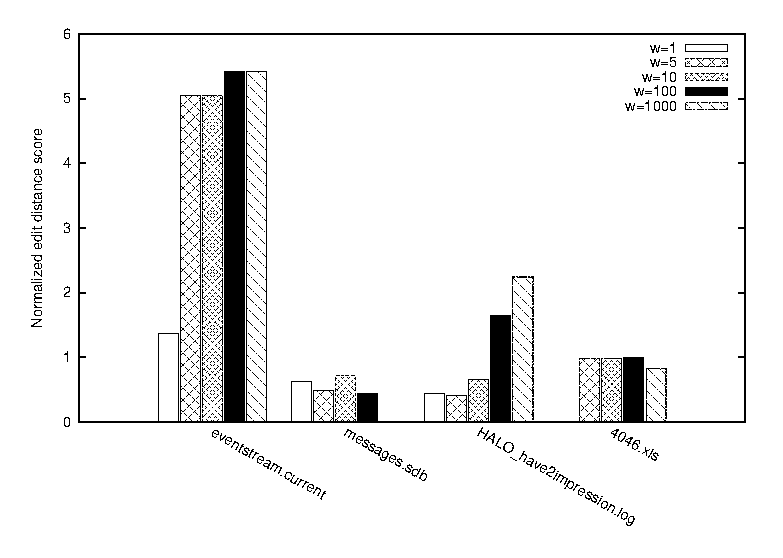
\includegraphics[width=\columnwidth]{adc}
\caption{Effects of $w$ on description quality}
\vskip -2ex
\label{fig:adc}
\end{figure}

To determine the effects of the weight $w$ in the MDL score on the quality
of the learning descriptions, we pick four smaller sources and learn
descriptions for them with $w$ set at 1, 5, 10, 100 and 1000, while
keeping the other parameters the same. The results in \figref{fig:adc}
show that setting $w$ to a very small or very large number either
results in bad descriptions with high edit distance score, or
timeouts at runtime (description was too complex to parse in reasonable time).
Therefore, we choose $w = 10$ for practicality.

To illustrate the quality of learned description and the difference between it
and the gold description, we show the gold description and the best
learned description of \cd{messages.sdb} in \figref{fig:gold-messages.sdb}
and \figref{fig:best-messages.sdb}. The learned description maintains a top-level
structure almost identical to the gold description, except the gold description
has slightly more refined details about the {\tt message\_t} type, which was
represented by {\tt Popt Struct\_6113} and the blob at the end.  The gold and learned descriptions 
for the other files are available on the web (\url{http://www.padsproj.org/incremental-learning.html}).

\begin{figure}[t]
\centering
{\footnotesize
\begin{code}
\kw{Pstruct} proc_id_t \{
        '[';
        Puint32 id;
        ']';
\};
\kw{Pstruct} daemon_t \{
        Pstring_SE (:"/[:\\[]/":) name;
        Popt proc_id_t v_proc_id;
        ':';
\};
\kw{Pstruct} msg_body_t \{
        daemon_t v_daemon_pri;
        Pwhite v_space;
        Pstring_SE(:Peor:) v_msg;
\};
\kw{Punion} message_t  \{
        msg_body_t v_normal_msg;
        Pstring_SE(:Peor:) v_other_msg;
\};
\kw{Precord} \kw{Pstruct} entry_t \{
        Pdate  v_date;
        ' ';
        Ptime v_time;
        ' ';
        Pstring(:' ':) v_id;
        ' ';
        message_t v_message;
\};
\kw{Psource} \kw{Parray} entries_t \{
        entry_t[];
\};
\end{code}
}\vskip -0.1ex
\caption{Gold description of messages.sdb}
\label{fig:gold-messages.sdb}
\end{figure}

\begin{figure}[t]
\centering
\vskip 2ex
{\footnotesize
\begin{code}
\kw{Pstruct} Struct_6113 \{
        Pstring(:':':)  v_blob_5869;
        ':';
\};
\kw{Precord} \kw{Pstruct} Struct_5671 \{
        Pdate  v_date_1;
        ' ';
        Ptime  v_time_6;
        ' ';
        Pstring (:' ':) v_string_33;
        ' ';
        Popt Struct_6113 v_opt_6096;
        Pstring_SE(:Peor:)  v_blob_6095;
\};
\kw{Psource} \kw{Parray} entries_t \{
        Struct_5671[];
\};
\end{code}
}\vskip -0.1ex
\caption{Best learned description of messages.sdb}
\label{fig:best-messages.sdb}
\end{figure}

